% !TEX root = atlas_iros_16.tex
%%%%%%%%%%%%%%%%%%%%%%%%%%%%%%%%%%%%%%%%%%%%%%%%%%%%%%%%%%%%%%%%%%%%%%%%%%%%%%%%
\subsection{Compliance Loss Compensation}
\label{sec:comp_obs}

\subsubsection{Loss of Compliance with Disturbance Compensation}
\label{sec:comp_obs_loss}
%
\begin{figure}
\centering
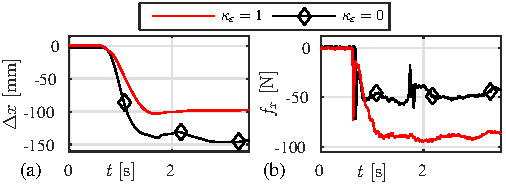
\includegraphics[]{./figures/ObserverStiff/ObsFeedthroughStiff_compare.pdf}
\caption{Position error $\Delta x$ and measured Cartesian external force $f_x$ are compared for two experiments with enabled ($\kappa_{\varepsilon}=1$) and disabled ($\kappa_{\varepsilon}=0$) disturbance compensation.
The end-effector was pushed manually and held at a certain displacement.}
\label{fig:stiff_observer_feedthrough}
\SkipBeforePicture
\end{figure}
%
The increased stiffness of the system, when using the disturbance compensation ($\kappa_{\varepsilon}=1$) was experimentally verified. For this, the robot end-effector was pushed with and without activated disturbance compensation, see Fig.~\ref{fig:stiff_observer_feedthrough}.
% Prozentuale Aussagen zu Kraft, Positionsfehler und Steifigkeit stammen aus ObserverFeedthroughStiff_Format.m
With enabled disturbance compensation the applied force was about $93$\% larger than without disturbance compensation (Fig.~\ref{fig:stiff_observer_feedthrough}~a) while the arm was only pushed back $67$\% in position (Fig.~\ref{fig:stiff_observer_feedthrough}~b).
This increased stiffness of about $187$\% is limited by the cutoff value for the estimated disturbance torque of $30$~Nm for safety reasons, as the observer was tuned to be near the (unknown) stability limit to ensure the fastest possible convergence.
However, with $\bm{K}_\mathrm{o}$ as chosen above, instabilities could not be observed during the experiments.

\subsubsection{Regaining Compliance with Force/Torque Sensing}
\label{sec:comp_obs_regain}
% Bild erstellt mit atlas_joint_impctrl_sqrt_damping_test_extforce_comp.m
\begin{figure}
\centering
\parbox{\columnwidth}{
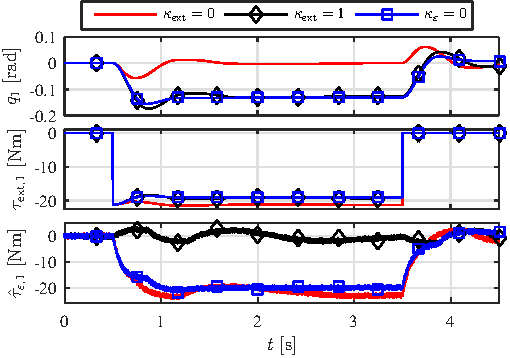
\includegraphics[width=\linewidth]{simulations/SimExp_ObsExtForce.pdf}
}
\vspace*{-1ex}
\caption{Simulation results: An external force step of 50~N is applied normal to the end-effector at $t=0.5~\mathrm{s}$ and released at $t=3.5~\mathrm{s}$.
Joint position $q_1$, external joint torque $\tau_{\mathrm{ext,1}}$, and observed disturbance torque $\hat{\tau}_{\varepsilon,1}$ are plotted for disabled disturbance compensation DC ($\kappa_\varepsilon=0$), DC without EFC ($\kappa_\mathrm{ext}=0$) and DC with EFC ($\kappa_\mathrm{ext}=1$).}
\label{fig:DistTorque}
\SkipBeforeText
\end{figure}
%
Since the wrist wrench sensor of the real system was not yet fully operational, the ability to eliminate external forces from the disturbance observer via (\ref{eqn:regainComp}) was validated in simulation.
The continuous time forward dynamics derived from (\ref{eqn:invdyn}) of the arm was implemented with viscous and Coulomb friction and parameters from Table~\ref{tab:errors_tracking_left}.
The observer gain was chosen to be uniformly $k_{\mathrm{o},i}=10~\mathrm{s}^{-1}$, stiffness $k_i=150~\mathrm{Nm/rad}$ and modal damping $d_{\xi,i}=0.3$.
The Controller (\ref{eqn:controller}) was implemented with model errors and sensor noise $\bm{\delta}$.
The model errors were generated with uniformly distributed pseudo random numbers between $\pm 10\%$ as a scaling factor to all masses, inertias, center of mass coordinates and friction coefficients.
The sensor noise was (component-wise) uniformly distributed between \mbox{$\pm 3.4\cdot10^{-4}~\mathrm{rad}$} for joint position, \mbox{$\pm 5.5\cdot10^{-2}~\mathrm{rad/s}$} for velocity, \mbox{$\pm 2\cdot10^{-4}~\mathrm{m/s^2}$} for the gravity vector, \mbox{$\pm 7.3\cdot10^{-2}~\mathrm{Nm}$} for the joint torque and \mbox{$\pm 2.3~\mathrm{N}$} for the external forces, respectively.
These values were obtained from the measurement data of the hydraulic joints during the starting phase of the experiment in Fig.~\ref{fig:stiff_observer_feedthrough}.

For this setup, a step change of the external force acting on the end-effector was performed with different observer settings.
The results are shown in Fig.~\ref{fig:DistTorque}.
For $\kappa_\varepsilon=0$, i.e. applying no disturbance compensation, compliant behavior is achieved. Using the disturbance compensation without EFC ($\kappa_\mathrm{ext}=0$) leads to a very stiff response according to (\ref{eqn:compLoss}), with $\hat{\tau}_{\varepsilon,1}$ converging to $\tau_{\mathrm{ext,1}}$.
When selecting $\kappa_\mathrm{ext}=1$, the observer torque remains near zero, as it only observes the model errors.
In addition, the compliance is the same as without disturbance compensation, i.e. as expected from (\ref{eqn:regainComp}).
Therefore, the simulation results imply, that this approach allows to compensate for model errors, while correctly reacting compliant to end-effector contacts at the same time.
%
\begin{figure}
\centering
\parbox{\columnwidth}{
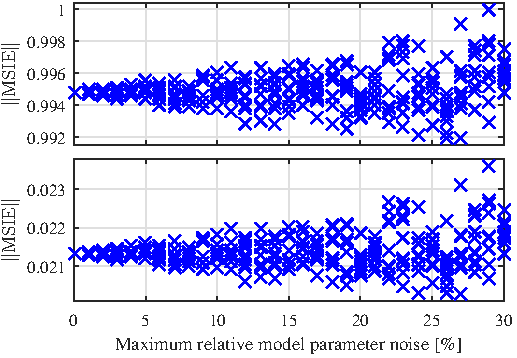
\includegraphics[width=\linewidth]{simulations/SimExp_MdlNoiseExtForce.pdf}
}
\caption{Simulation results: The experiment of Fig.~\ref{fig:DistTorque} was done multiple times with different model errors.
The normalized mean squared integrated error is plotted over the maximum parameter noise level.
The results for $\kappa_\mathrm{ext}=0$ and $\kappa_\mathrm{ext}=1$ are shown in the top and the bottom plot respectively.}
\label{fig:MdlNoise}
\SkipBeforePicture
\vspace*{-1ex}
\end{figure}
%
\begin{figure}
\centering
\parbox{\columnwidth}{
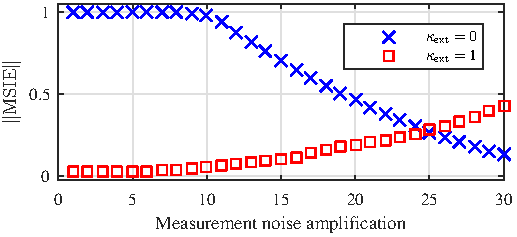
\includegraphics[width=\linewidth]{simulations/SimExp_MesNoiseExtForce.pdf}
}
\caption{Simulation results: The experiment from Fig.~\ref{fig:DistTorque} was done multiple times with different measurement errors.
The normalized mean squared error is depicted over the scaling factor applied to all measurement noise levels from the simulation of Fig.~\ref{fig:DistTorque}.}
\label{fig:MesNoise}
\SkipBeforeText
\end{figure}
%
\subsubsection{Robustness of Disturbance Compensation with EFC against Model Errors}
Further simulations (as in Fig.~\ref{fig:DistTorque}) were performed to investigate the robustness of the above method.
First, the influence of model errors is investigated.
The model errors were introduced by scaling the masses, the center of gravity positions of the links, the link inertias and the friction parameters by uniformly distributed random factors.
The normalized mean squared integrated error (MSIE)
\begin{equation}
\mathrm{MSIE}=\frac{1}{n_{\mathrm{j}}T_\mathrm{f}}\sum_{i=1}^{n_{\mathrm{j}}}\int_0^{T_\mathrm{f}} \left(q_i(t)-q_i^{\mathrm{ref}}(t)\right)^2\mathrm{d}t
\end{equation}
is depicted over the maximum noise factor for limits from 1\% to 30\% in Fig.~\ref{fig:MdlNoise} for the controller with and without EFC.
The norm $\|\mathrm{MSIE}\|=\mathrm{MSIE}/\max(\mathrm{MSIE})$ is calculated for Fig.~\ref{fig:MdlNoise} and Fig.~\ref{fig:MesNoise} separately.
The compliant behavior of the controller without disturbance compensation and without model errors or measurement noise was selected as reference $\bm{q}^\mathrm{ref}$.
In order to gain comparable results, the model errors were the same in both plots.
It can be seen that the influence of the model errors is similar for both cases and the results with EFC remain close to the reference case. The order of magnitude between the results with and without EFC stays the same for all model error levels.
%Therefore, the deviation from the desired compliant behavior increases slightly
Even with an identification error of up to $30\%$, the controller can cope with the resulting model errors for this quasi-static movement.

\subsubsection{Robustness of Disturbance Compensation with EFC against Sensor Noise}

Figure~\ref{fig:MesNoise} depicts the influence of measurement noise on controller performance.
The measurement noise levels from above were scaled by factors of 1 to 30 and the MSIE is compared for the controller with ($\kappa_\mathrm{ext}=1$) and without EFC ($\kappa_\mathrm{ext}=0$).
It can be seen that for noise levels amplified up to 10 times, the deviation from the reference behavior does not change noticeably in either case, i.e. the compliance rendering of the controller remains the same despite increased noise.

For larger measurement noise the deviation from the desired behavior becomes smaller for $\kappa_\mathrm{ext}=0$ since the limitation of the observer output prevents the compensation of external forces for high measurement noise.
This effect even leads to a behavior closer to the desired one with \mbox{$\kappa_\mathrm{ext}=0$} instead of \mbox{$\kappa_\mathrm{ext}=1$} for very high measurement noise (at least 25 times as high as observed in the experiments).
In term, Fig.~\ref{fig:MesNoise} implies that the controller is able to cope with measurement noise about 10 times higher than found in our experimental setup.
To cope with larger measurement noise, one would have to use filtering or increase the output limit of the observer.